\chapter{燃烧：火需要什么}\label{ch:g4:what-a-fire-needs}

黄昏时的篝火。它需要干木柴、一根用来点火的火柴，
以及吹过火堆、让火焰保持明亮的风。过了一小时，木柴
已烧成发光的余烬和白色的灰，灰色的烟飘散了，
飘向天空。木柴去哪儿了？火需要什么，
又留下了什么？

\begin{recall}
空气是多种气体的混合物：约五分之四是氮气，五分之一是氧气，
还有少量氩气和二氧化碳。火焰从周围的空气中获取氧气；
罩在广口瓶下的蜡烛，在剩余氧气太少时就会熄灭
（见\cref{ch:g4:air-a-mixture-of-gases}）。
\end{recall}

\begin{omfigure}
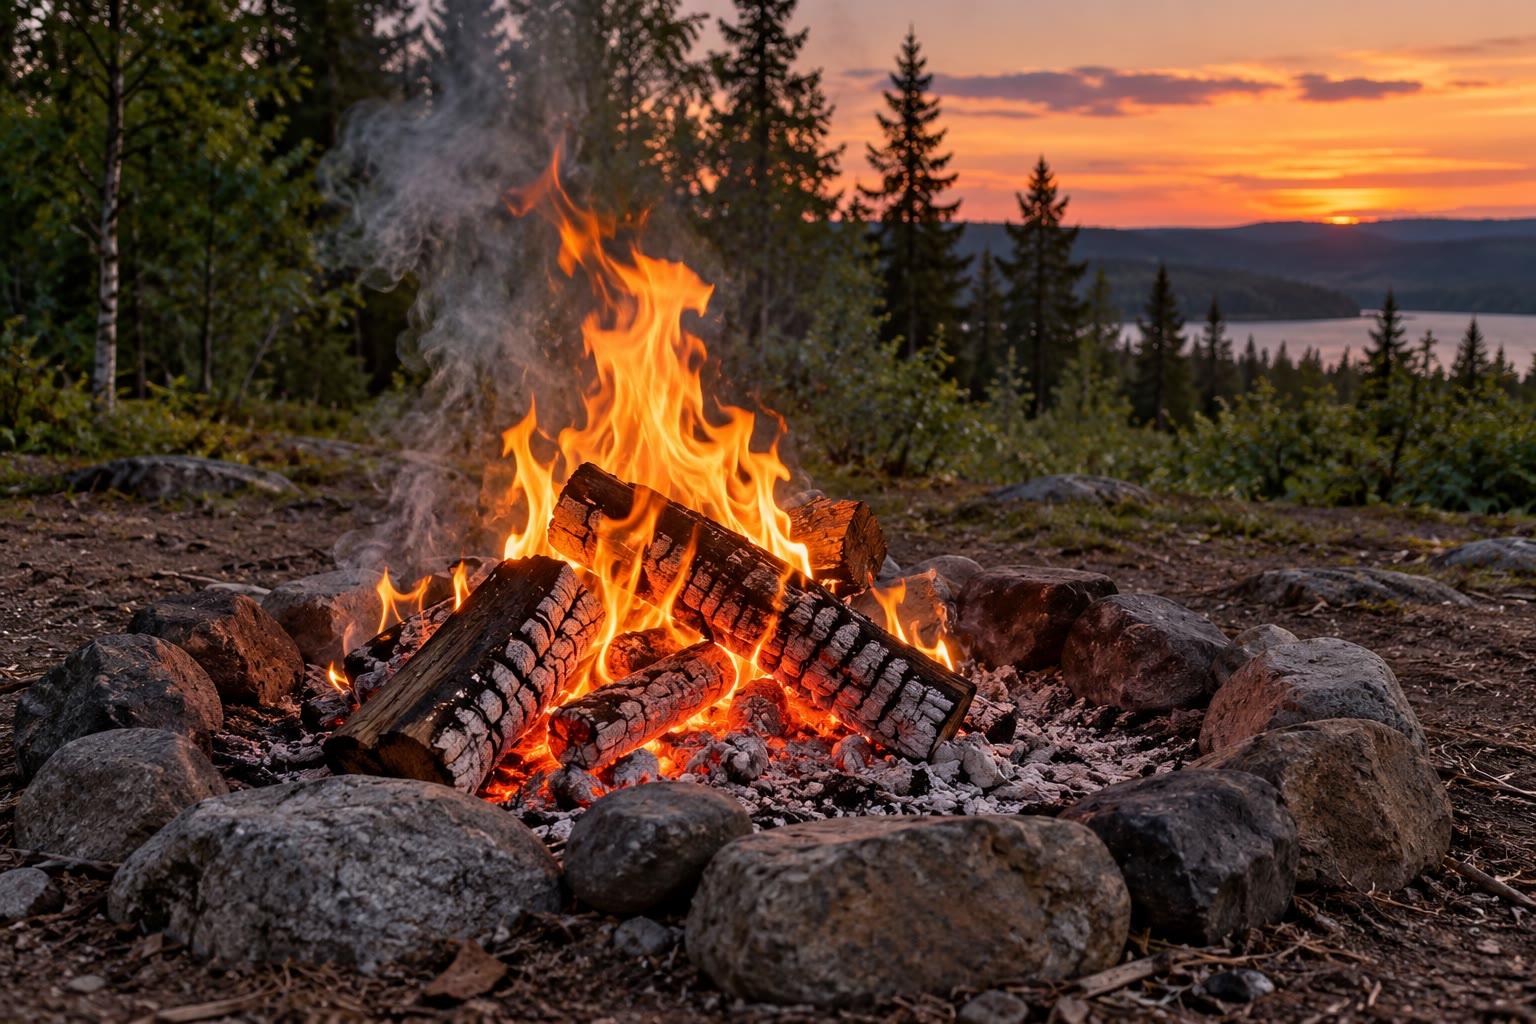
\includegraphics[width=0.6\linewidth]{images/book1/ai/g4-campfire.jpg}

{\small 篝火：木柴、空气和火柴——之后是灰烬和
烟。}
\end{omfigure}

\section{燃料}

\begin{definition}[燃料]\label{def:g4:what-a-fire-needs:fuel}
\emph{燃料}\index{燃料}是能够燃烧并放出热和光的材料：
木柴、纸、煤、石蜡、灶具用的燃气、汽油、
取暖油。
\end{definition}

\begin{example}[固体、液体和气体燃料]\label{ex:g4:what-a-fire-needs:fuels}
木柴、纸、煤和石蜡是固体燃料。汽油和取暖油
是液体燃料。厨房灶具的燃气和打火机中的气体
是气体燃料。
\end{example}

\begin{remark}[并非所有东西都能燃烧]\label{rem:g4:what-a-fire-needs:not}
石头、沙子、玻璃和水都不能燃烧，它们不是燃料。这就是
壁炉要用石头或砖砌成、而沙子和水可以用来灭火的原因。
用来灭火。
\end{remark}

\section{燃烧三要素}

\begin{definition}[燃烧三要素]\label{def:g4:what-a-fire-needs:fire-triangle}
火的燃烧同时需要三个条件：燃料、空气中的氧气，
以及使其开始燃烧的热。这三者被画成一个三角形的三条边，
这个三角形称为\emph{燃烧三要素}\index{燃烧三要素}。若缺少其中一边，
就不会有火。
\end{definition}

\begin{omfigure}
\begin{tikzpicture}[font=\small]
  \coordinate (A) at (0,0); \coordinate (B) at (5,0); \coordinate (C) at (2.5,4.1);
  \draw[line width=3pt, brown!70!black] (A) -- (B);
  \draw[line width=3pt, omDef] (B) -- (C);
  \draw[line width=3pt, red!75!black] (C) -- (A);
  \node[below=4pt, font=\small\bfseries, brown!60!black] at (2.5,0) {燃料};
  \node[right=4pt, font=\small\bfseries, omDef] at (3.75,2.05) {氧气（来自空气）};
  \node[left=4pt, font=\small\bfseries, red!75!black] at (1.25,2.05) {热（引燃）};
  % a flame in the middle
  \fill[orange!80] (2.5,0.55) .. controls (1.95,1.15) and (2.35,1.75) .. (2.55,2.3)
    .. controls (2.75,1.75) and (3.05,1.15) .. (2.5,0.55);
  \fill[yellow!80] (2.5,0.7) .. controls (2.25,1.05) and (2.4,1.35) .. (2.52,1.65)
    .. controls (2.62,1.35) and (2.75,1.05) .. (2.5,0.7);
\end{tikzpicture}

{\small 燃烧三要素：燃料、氧气和热，三者缺一不可。}
\end{omfigure}

\begin{example}[点燃火柴]\label{ex:g4:what-a-fire-needs:match}
火柴头在火柴盒的侧面摩擦。摩擦使它温度升高，
达到足以开始燃烧的程度，这正是燃烧三角形中的热。火柴
杆是燃料，空气提供氧气。
\end{example}

\begin{example}[对余烬吹气]\label{ex:g4:what-a-fire-needs:embers}
看似快要熄灭的发光余烬，被人吹一吹，
又会重新燃起火焰：吹气带来更多空气，也就带来更多氧气，
送到仍然炽热的燃料上。
\end{example}

\section{燃烧会生成新物质}

\begin{definition}[燃烧]\label{def:g4:what-a-fire-needs:burning}
\emph{燃烧}\index{燃烧}是指燃料从空气中获取氧气
并放出热和光的过程。化学上也把它叫做
\emph{燃烧}\index{燃烧}。燃烧时燃料和
氧气都被耗尽，并生成新的物质：烟、灰、二氧化碳
和水蒸气。
\end{definition}

\begin{proposition}[燃烧不可逆转]\label{prop:g4:what-a-fire-needs:new}
火燃烧后剩下的灰烬和烟，无论等待多久，都不会变回木柴。
燃烧会生成原来不存在的新物质，燃料
就永远消失了。
\end{proposition}

\begin{inthelab}[蜡烛上方的冷玻璃烧杯]
老师把一只冷的、干燥的玻璃烧杯倒扣着，在蜡烛火焰上方
停留片刻。玻璃杯内壁会凝结出许多细小的水珠：
这是燃烧的蜡烛产生的水蒸气，在冷玻璃上
重新变成了液体。燃烧的蜡烛会生成水，也会生成二氧化碳，
这可以用后面章节将学到的检验方法来检测。
\end{inthelab}

\begin{omfigure}
\begin{tikzpicture}[font=\small, scale=1.3]
  % candle
  \fill[white, draw=black!50] (-0.25,0) rectangle (0.25,1.2);
  \draw[black!70] (0,1.2) -- (0,1.33);
  \fill[orange!85] (0,1.3) .. controls (-0.16,1.5) and (-0.06,1.75) .. (0,1.95)
    .. controls (0.06,1.75) and (0.16,1.5) .. (0,1.3);
  \fill[yellow!85] (0,1.36) .. controls (-0.08,1.5) and (-0.03,1.62) .. (0,1.72)
    .. controls (0.03,1.62) and (0.08,1.5) .. (0,1.36);
  % upturned cold beaker above
  \pic[transform shape, rotate=180] at (0,4.3) {beaker={0}{white}};
  \foreach \x/\y in {-0.6/3.9,-0.45/4.1,-0.2/3.95,0.1/4.15,0.35/3.9,0.6/4.05,
                     -0.7/3.5,0.7/3.4,-0.72/3.0,0.72/2.9}
    \fill[omDef!55] (\x,\y) circle (0.035);
  \draw[<-, omProp, thick] (0.68,3.95) -- (2.0,4.2) node[right, text=black]
    {水滴};
  \draw[<-, omProp, thick] (0.85,3.2) -- (2.0,3.3) node[right, text=black]
    {冷玻璃杯，倒扣};
  \draw[<-, omProp, thick] (0.15,1.7) -- (2.0,1.9) node[right, text=black]
    {火焰：石蜡燃烧};
  \draw[<-, omProp, thick] (0.3,0.6) -- (2.0,0.7) node[right, text=black]
    {石蜡：燃料};
\end{tikzpicture}

{\small 冷玻璃杯放在蜡烛上方时会起雾：燃烧的石蜡
会产生水蒸气。}
\end{omfigure}

\begin{example}[木柴会变成什么]\label{ex:g4:what-a-fire-needs:log}
一根重几千克的木柴燃烧后，只剩下一小堆灰烬。
大部分木材并没有消失：它与空气中的氧气结合，
变成了烟、二氧化碳和水蒸气，这些都是气体，
飘散到空中。
\end{example}

\section{灭火}

\begin{method}[灭火：去掉一个要素]\label{met:g4:what-a-fire-needs:out}
要灭火，就要去掉燃烧三要素中的一个：
\begin{itemize}
  \item \textbf{隔绝氧气}：用灭火毯、锅盖或沙子盖住火焰，
        使空气无法接触火焰；
  \item \textbf{带走热量}：向燃烧的木材或纸张上浇水，
        使其温度降到无法继续燃烧的程度以下；
  \item \textbf{移走燃料}：关掉煤气阀门，或清除
        森林火灾周围的干枯植物。
\end{itemize}
\end{method}

\begin{omfigure}
\begin{tikzpicture}[font=\small, scale=0.7]
  \foreach \k/\lab/\side in {0/{毯子：隔绝氧气}/1, 1/{水：降低温度}/2,
                              2/{关闭燃气：移除燃料}/0} {
    \begin{scope}[xshift=\k*6.2cm]
      \coordinate (A) at (0,0); \coordinate (B) at (4,0); \coordinate (C) at (2,3.3);
      \pgfmathsetmacro\oa{\side==0 ? 0.2 : 1}
      \pgfmathsetmacro\ob{\side==1 ? 0.2 : 1}
      \pgfmathsetmacro\oc{\side==2 ? 0.2 : 1}
      \draw[line width=2.5pt, brown!70!black, opacity=\oa] (A) -- (B);
      \draw[line width=2.5pt, omDef, opacity=\ob] (B) -- (C);
      \draw[line width=2.5pt, red!75!black, opacity=\oc] (C) -- (A);
      \ifnum\side=0 \draw[line width=1.4pt, black] (1.6,-0.4) -- (2.4,0.4) (1.6,0.4) -- (2.4,-0.4);\fi
      \ifnum\side=1 \draw[line width=1.4pt, black] (2.6,1.25) -- (3.4,2.05) (2.6,2.05) -- (3.4,1.25);\fi
      \ifnum\side=2 \draw[line width=1.4pt, black] (0.6,1.25) -- (1.4,2.05) (0.6,2.05) -- (1.4,1.25);\fi
      \node[align=center, anchor=north] at (2,-0.6) {\lab};
    \end{scope}
  }
\end{tikzpicture}

{\small 三种灭火方法，每种各去掉燃烧三角形中的一边
（图中打叉的部分）：氧气、热量或燃料。}
\end{omfigure}

\begin{omfigure}
\begin{minipage}[t]{0.48\linewidth}\centering
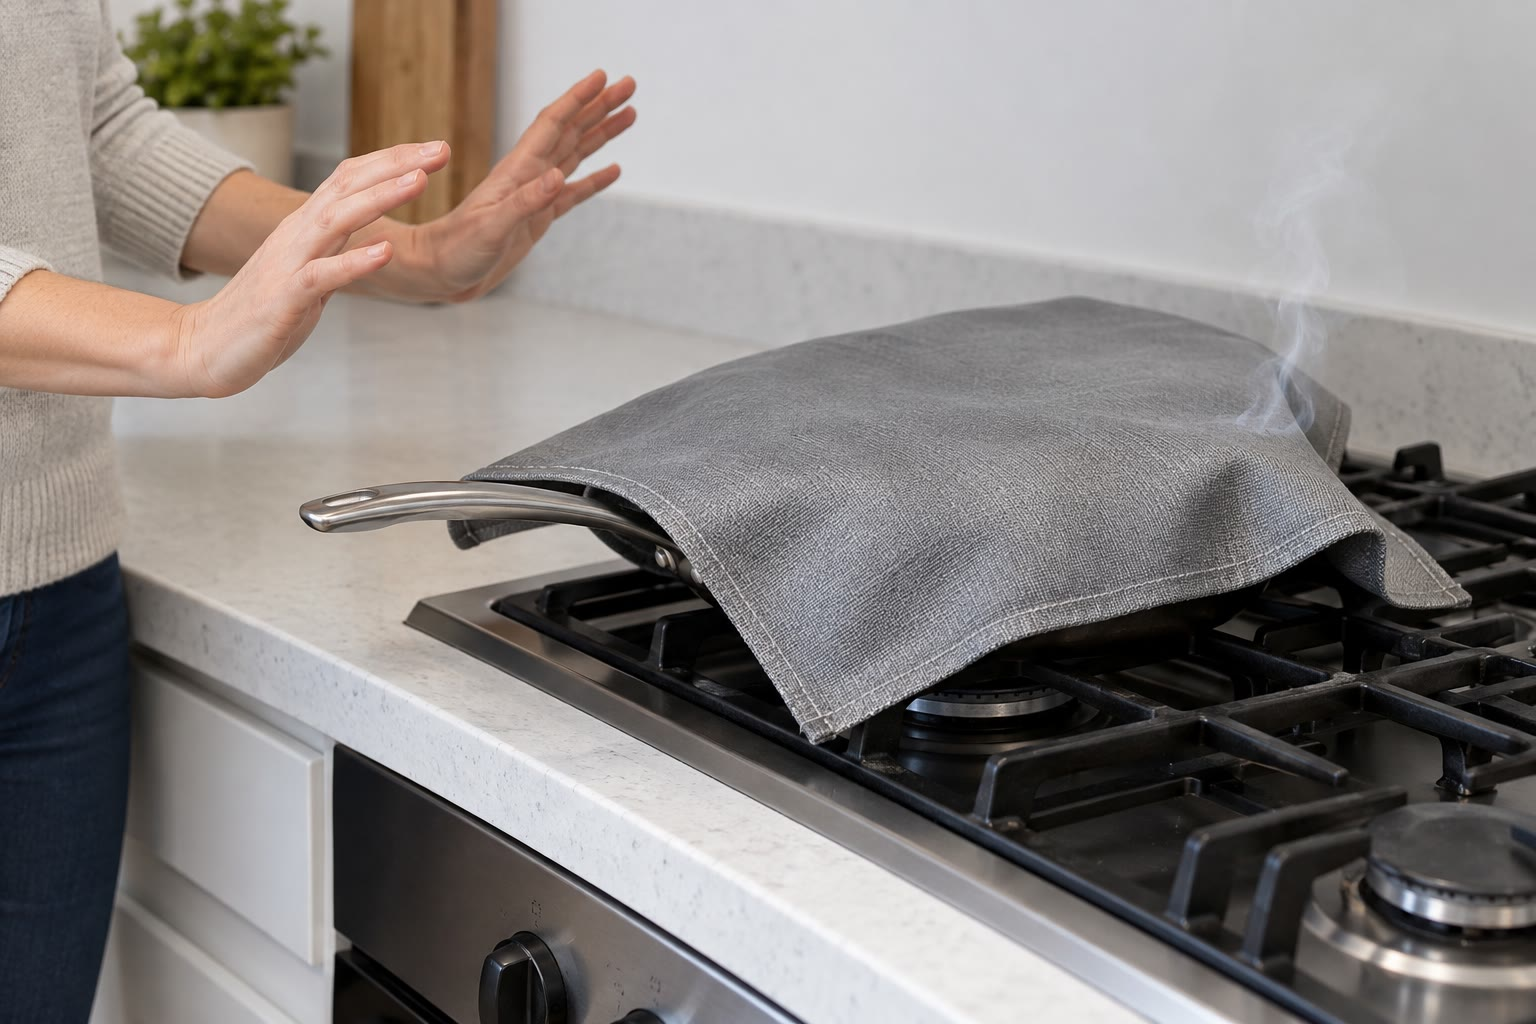
\includegraphics[width=\linewidth,height=4.6cm,keepaspectratio]{images/book1/ai/g4-fire-blanket.jpg}

{\small 灭火毯盖在平底锅上：空气无法再接触
火焰。}
\end{minipage}\hfill
\begin{minipage}[t]{0.48\linewidth}\centering
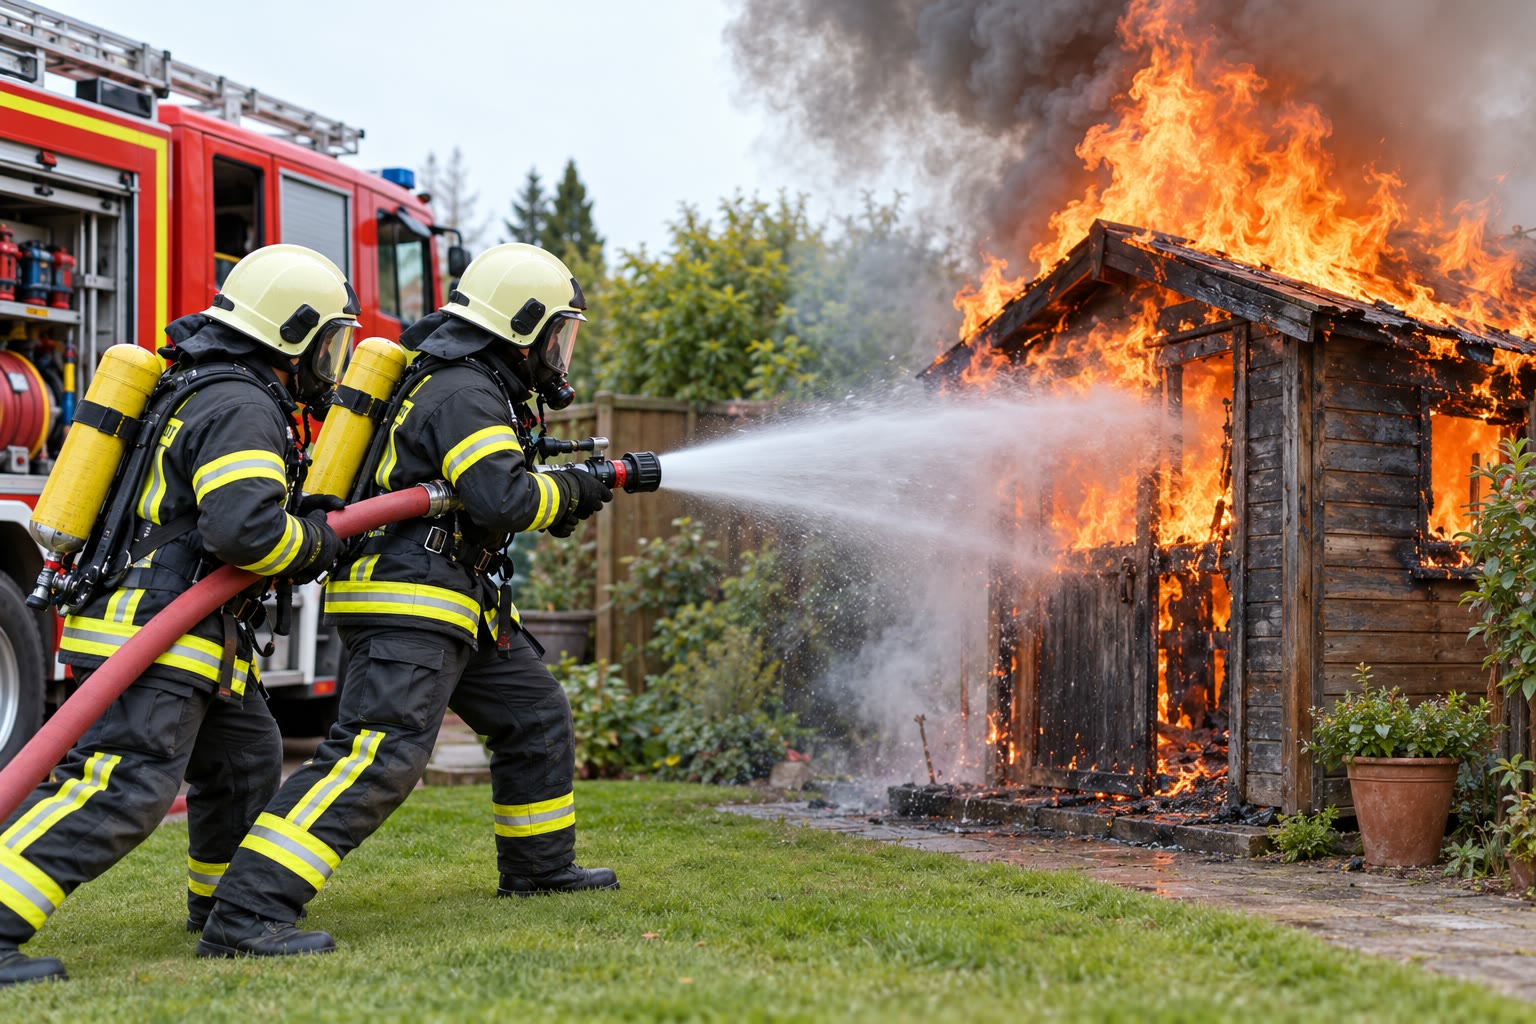
\includegraphics[width=\linewidth,height=4.6cm,keepaspectratio]{images/book1/ai/g4-firefighters.jpg}

{\small 消防员向燃烧的棚屋喷水降温。}
\end{minipage}
\end{omfigure}

\section{火灾安全}

\begin{remark}[油锅着火时绝不能浇水]\label{rem:g4:what-a-fire-needs:oil}
若煎锅中的油着火，任何人都不能向锅里泼水，
因为水会立即在油层下沸腾，把燃烧的油溅出锅外。
应由成年人关闭煤气或电炉，并用锅盖或灭火毯
盖住油锅。
\end{remark}

\begin{safety}{\ghs{GHS02}\ghs{GHS04}}
% ledger: ghs:butane
打火机或露营气罐中的气体是丁烷。其火焰
图标（GHS02）表示：极易燃，远离火焰与
火花。气瓶图标（GHS04）表示：
气体处于高压之下。
\end{safety}

\begin{proposition}[发生火灾时怎么办]\label{prop:g4:what-a-fire-needs:safety}
烟雾是火灾中的第一大危险：它有高温，会遮住逃生的路，
且吸入有毒。天花板上的烟雾报警器
一遇到烟雾就会大声鸣叫。若发生火灾：迅速撤离，
在烟雾下方低身前行，随手关上身后的门，并在
屋外拨打消防电话。千万不要再返回屋内。
\end{proposition}

\begin{omfigure}
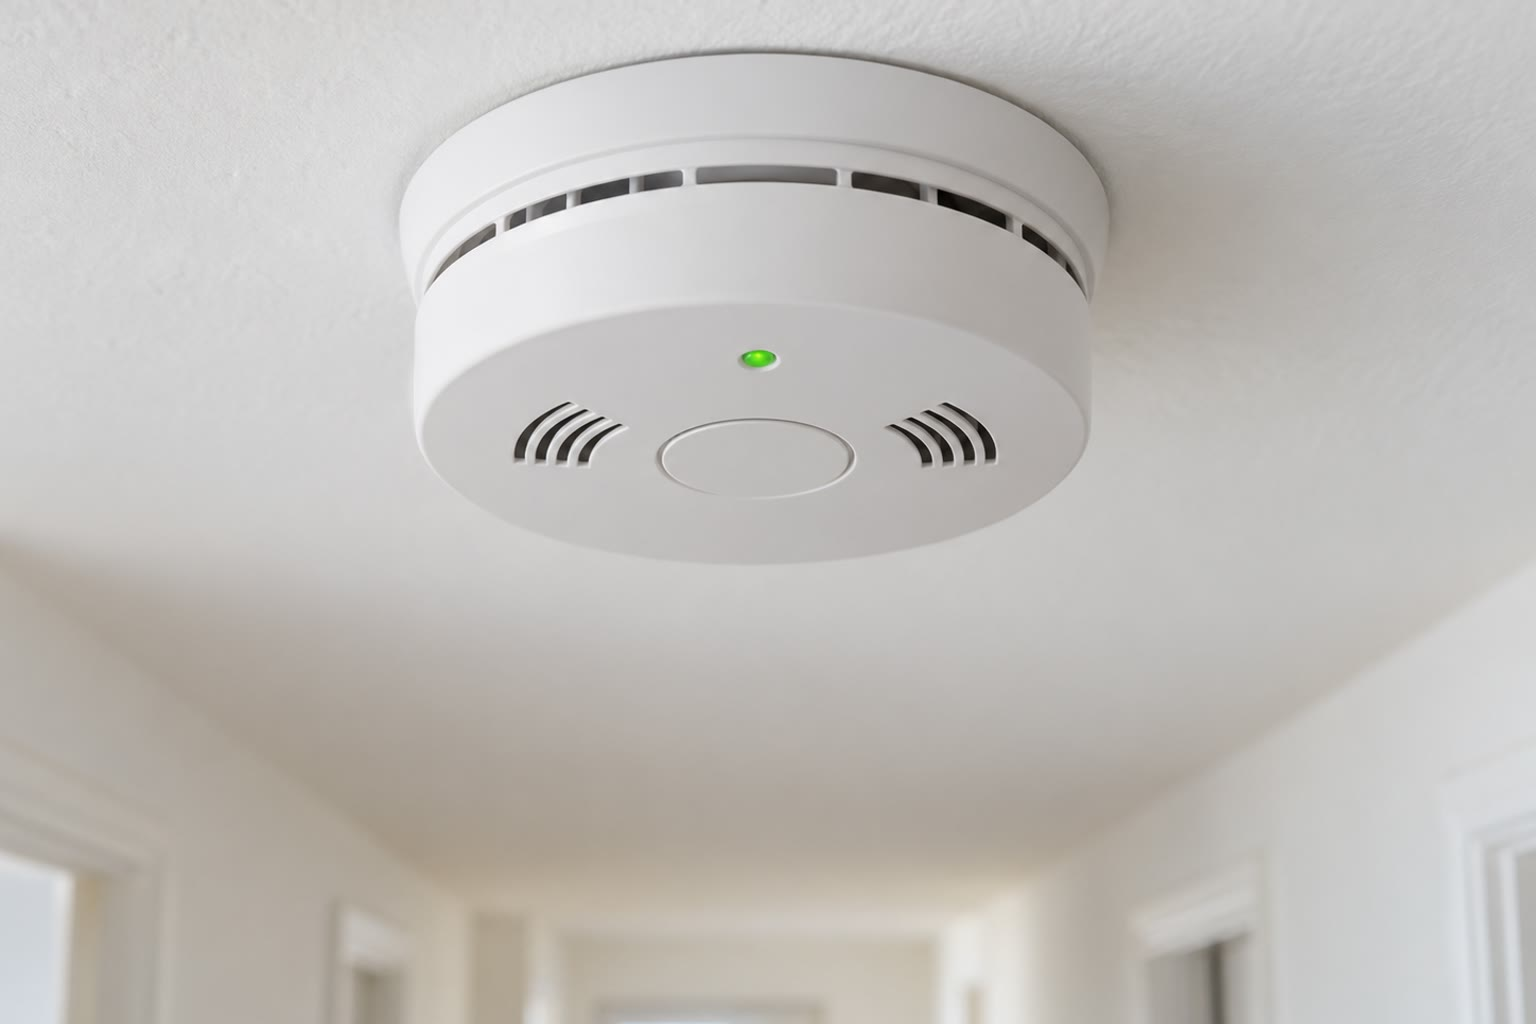
\includegraphics[width=0.42\linewidth]{images/book1/ai/g4-smoke-alarm.jpg}

{\small 烟雾报警器：一遇到烟雾就会鸣响。}
\end{omfigure}

\section{练习}

\begin{exercise}[$\star$]\label{exo:g4:what-a-fire-needs:1}
说出燃烧三要素。
\end{exercise}

\begin{exercise}[$\star$]\label{exo:g4:what-a-fire-needs:2}
下列物质中哪些是燃料：木材、沙子、石蜡、玻璃、汽油、水、
纸张？
\end{exercise}

\begin{exercise}[$\star$]\label{exo:g4:what-a-fire-needs:3}
将灭火毯盖在一小团火上，它去掉了
燃烧三要素中的哪一个？
\end{exercise}

\begin{exercise}[$\star$]\label{exo:g4:what-a-fire-needs:4}
消防员向着火的棚屋喷水。
水去掉了燃烧三要素中的哪一个？
\end{exercise}

\begin{exercise}[$\star$]\label{exo:g4:what-a-fire-needs:5}
说出木材燃烧时生成的三种新物质。
\end{exercise}

\begin{exercise}[$\star$]\label{exo:g4:what-a-fire-needs:6}
为什么对着发红的余烬吹气，它们会重新燃烧起来？
\end{exercise}

\begin{exercise}[$\star$]\label{exo:g4:what-a-fire-needs:7}
把一只冷玻璃杯放在蜡烛上方，杯子会起雾。
蜡烛生成了哪种新物质？
\end{exercise}

\begin{exercise}[$\star$]\label{exo:g4:what-a-fire-needs:8}
如果烟雾报警器响起并看到冒烟，你首先应该做什么？
\end{exercise}

\begin{exercise}[$\star$]\label{exo:g4:what-a-fire-needs:9}
看一看这幅有三个小三角形的图，
关闭燃气时，哪一个被划掉了？
\end{exercise}

\begin{exercise}[$\star\star$]\label{exo:g4:what-a-fire-needs:10}
为了阻止森林火灾蔓延，消防员有时会在火前
砍掉一条宽阔的林带。他们去掉的是
燃烧三要素中的哪一个？
\end{exercise}

\begin{exercise}[$\star\star$]\label{exo:g4:what-a-fire-needs:11}
一根原木的质量远大于其灰烬。原木的一部分是否消失了？
请解释它去了哪里。
\end{exercise}
